%Author(s), Course variables
\newcommand{\titl}{Januarprojekt}
\newcommand{\authone}{Abinav Aleti}
\newcommand{\SIDone}{s224786}
\newcommand{\authtwo}{Yahya Alwan}
\newcommand{\SIDtwo}{s224739}
\newcommand{\auththree}{Aslan Behbahani}
\newcommand{\SIDthree}{s224819}
\newcommand{\authfour}{Rasmus Wiuff}
\newcommand{\SIDfour}{s163977}
\newcommand{\courseno}{02121}
\newcommand{\course}{Introduktion til Softwareteknologi}
\newcommand{\lb}{\\}
%Basics
\documentclass[a4paper, danish]{article}
\usepackage[utf8]{inputenc}
\usepackage{babel}
\usepackage[moderate]{savetrees}
%Symbols and scientifics
\usepackage{amsmath, amsfonts, amssymb, bm}
\numberwithin{equation}{section}
\usepackage{physics}
\usepackage{mathtools}
\usepackage{siunitx}
\sisetup{
    per-mode = power ,
    round-mode = figures ,
    round-precision = 3 ,
    scientific-notation = false ,
    output-decimal-marker = {.} ,
    exponent-product = \times ,
    separate-uncertainty = true ,
    uncertainty-separator = \ ,
    range-phrase = - ,
    range-units =  single ,
    inter-unit-product = \ensuremath{{\cdot{}}} ,
    number-unit-product = \ ,
    multi-part-units = single ,
}

%Appendix, TOC and Bibliography
\usepackage{appendix}
\renewcommand\appendixtocname{Appendicer}
\usepackage[nottoc]{tocbibind}
\setcounter{tocdepth}{2}
\usepackage{lastpage}

%Figures
\usepackage[svgnames]{xcolor} % Required to specify font color
\usepackage{float}
\usepackage{graphicx}
    \graphicspath{{Graphics/}}
\usepackage{setspace}
\usepackage{listings}
\usepackage{subcaption}
\usepackage[format=plain,
    labelfont={bf,it,footnotesize},
    textfont={it,footnotesize}]{caption}
% \captionsetup[table]{name=Huskeord}
\captionsetup{font={stretch=0.9}}
\usepackage{wrapfig}
\usepackage[a4paper, centering, rmargin=2.5cm, tmargin=2.5cm, lmargin=2.5cm, bmargin=3.5cm]{geometry}
\usepackage{etoolbox}
\usepackage{verbatim}
\usepackage[space]{grffile}
\usepackage[final]{pdfpages}
\usepackage{array}
\usepackage{multirow}
\usepackage{dcolumn}
\usepackage{fontawesome}
\usepackage{pgfgantt}
\usepackage{tikz}
\usetikzlibrary{positioning}
\newcommand{\ttt}[1]{\texttt{#1}}
\newcommand{\F}{\mathtt{F}}
\newcommand{\T}{\mathtt{T}}

\newcommand{\lorf}{\ensuremath{\lor\F}}
\newcommand{\lort}{\ensuremath{\lor\T}}
\newcommand{\landf}{\ensuremath{\land\F}}
\newcommand{\landt}{\ensuremath{\land\T}}
\newcommand{\tof}{\ensuremath{\to\!\F}}
\newcommand{\tot}{\ensuremath{\to\!\T}}
\newcommand{\lrf}{\ensuremath{\leftrightarrow\!\F}}
\newcommand{\lrt}{\ensuremath{\leftrightarrow\!\T}}
\newcommand{\negf}{\ensuremath{\neg\F}}
\newcommand{\negt}{\ensuremath{\neg\T}}
\newcommand{\allf}{\ensuremath{\forall\F}}
\newcommand{\allt}{\ensuremath{\forall\T}}
\newcommand{\exf}{\ensuremath{\exists\F}}
\newcommand{\ext}{\ensuremath{\exists\T}}

\newcommand{\first}[2]{\node (root) {\textcolor{red}{\scriptsize 1} \(#1\) : \texttt{#2}};}
\newcommand{\formula}[4]{\node (#1) [#2] {\textcolor{red}{\scriptsize #1} \(#3\) : \texttt{#4}};}
\newcommand{\branch}[2]{\path (#1) edge[-] (#2);}
\newcommand{\rbranch}[4]{\path (#3) edge[-] node [midway, right, blue] {\(#1\) på \(#2\)} (#4);}
\newcommand{\closed}[2]{\node (#1) [below = .1em of #2] {\(\times\)};}
\newcommand{\open}[2]{\node (#1) [below = .1em of #2] {\(\bigcirc\)};}
\newenvironment{tableau}{\begin{tikzpicture}[node distance = .5pt]}{\end{tikzpicture}}

%Header footer
\usepackage{fancyhdr}
\pagestyle{fancy}
\lhead{\titl \lb Kursus \courseno \lb \course \lb 20. januar 2023}
\chead{
\includegraphics[height=42.5pt]{DTU}}
\rhead{\authone \ \textbf{\SIDone} \lb \authtwo \ \textbf{\SIDtwo} \lb \auththree \ \textbf{\SIDthree} \lb \authfour \ \textbf{\SIDfour}}
\cfoot{Side \thepage\, af \pageref*{LastPage}}
\renewcommand{\headrulewidth}{0.4pt}
\renewcommand{\footrulewidth}{0.4pt}
\setlength{\headheight}{46.54448pt}
\addtolength{\topmargin}{-9.79414pt}

%Text tools
\usepackage{parcolumns}
\usepackage[super]{nth}
\usepackage[normalem]{ulem}
\usepackage{import}
\usepackage{url}
\usepackage{lipsum}
\usepackage{microtype}
\usepackage[pdfencoding=auto, psdextra]{hyperref}
\hypersetup{
    colorlinks   = true, %Colours links instead of ugly boxes
    urlcolor     = blue, %Colour for external hyperlinks
    linkcolor    = blue, %Colour of internal links
    citecolor   = red %Colour of citations
}
\usepackage[capitalise]{cleveref}
% \crefname{table}{Huskeord}{Huskeord}
\usepackage{enumitem}
\newlist{arrowlist}{itemize}{1}
\setlist[arrowlist]{label={\(\rightarrow\)}}
\usepackage{booktabs}
\usepackage{todonotes}
\usepackage{silence}
\usepackage[square, longnamesfirst, numbers]{natbib}
\usepackage{empheq}
\usepackage{minted}
\setminted{fontsize=\small,
           linenos=true}
\usemintedstyle{tango}
\renewcommand{\listoflistingscaption}{Listings}
\newcommand{\im}[3]{\inputminted[linenos=true, python3=true, firstline=#2, lastline=#3]{python}{#1}}
\newcommand{\java}[3]{\inputminted[linenos=true, firstline=#2, lastline=#3]{java}{#1}}
\usepackage{tabularx}

%Definitions and new commands
\newcommand{\degr}{^{\circ}}
\newcommand{\me}{\mathrm{e}}
\newcommand*\mathinhead[2]{\texorpdfstring{\(\boldsymbol{#1}\)}{#2}}

%Title and sectioning
\def\Vhrulefill{\leavevmode\leaders\hrule height 0.7ex depth \dimexpr0.4pt-0.7ex\hfill\kern0pt}
\usepackage{titlesec}
\definecolor{DTUred}{cmyk}{0, .91, .72, .23}
\definecolor{FMNgrey}{cmyk}{.73,.43,.53,.38}
\newcolumntype{a}{>{\columncolor{gray}}c}
%Use letters insted of numbers in section numbering
% \renewcommand{\thesection}{\Alph{section}}
% \renewcommand{\thesubsection}{\Alph{subsection}}
\usepackage{titling}

\makeatletter
\newcommand{\github}[1]{%
   \href{#1}{\color{DTUred}\faGithub}%
}
\makeatother

\begin{document}

\titleformat{\section}[block]
{\normalfont\Large\scshape\filright\color{DTUred}}{\fbox{\thesection}}{1em}{}

\titleformat{\subsection}
{\titlerule
    \vspace{.8ex}%
    \normalfont\scshape\color{FMNgrey}}
{\thesubsection.}{.5em}{}

\title{
\includegraphics[width=.5\textwidth]{icon.eps}\lb\vspace{.5em}\Huge\scshape\color{DTUred} \titl\lb\vspace{-4mm}\rule{4cm}{0.5mm}\lb\Large{\courseno \ \course}}
\preauthor{\begin{center}
    \large \lineskip 0.5em%
    \begin{tabular}[t]{r}}
\author{\textbf{Afleveringsgruppe 16:} \lb \lb \authone \ \textbf{\SIDone} \lb \authtwo \ \textbf{\SIDtwo} \lb \auththree \ \textbf{\SIDthree} \lb \authfour \ \textbf{\SIDfour} \lb \href{https://github.com/rwiuff/Reversi}{\color{DTUred}github.com/rwiuff/Reversi} \github{https://github.com/rwiuff/Reversi}}
\postauthor{\end{tabular}\par\end{center}}
\date{20. januar 2023}
\maketitle
\thispagestyle{empty}
\pagenumbering{arabic}
\setcounter{page}{0}
\newpage
\tableofcontents
\addtocontents{toc}{~\hfill\textbf{Side}\par}
\thispagestyle{empty}
\setcounter{page}{0}
\newpage
\setcounter{page}{1}

% !TeX root = ..\G16.tex
\section{Introduktion \& Problemanalyse}
\subsection{Arbejdsfordeling}
Arbejdsfordelingen under projektet kan ses i \cref{sec:arbejde}.
\subsection{Opgaven}
I dette projekt har vi skulle skrive et program, der starter- og kører spillet "Reversi", et brætspil der handler om kontrollere et bræt med flest mulige brikker. Programmet skal være skrevet i JavaFX. 
Problemet består i at, via. diverse datastrukturer, at skulle beskrive et bræt, brikkerne såvel som deres egenskaber og opførsel. Der har skulle være en grænseflade, der giver udtryk for alt det visuelle, såvel som logikken, der binder de forskellige elementer sammen. 
Vi har som hjælp til at designe programmet benyttet os af Model-View-Control-strukturen. Vi har skrevet modellen, som er logikken bag alle reaktioner, programmet kan have til diverse handlinger, vi har skrevet view, som er det grafiske element, der bestemmer hvordan programmet skal se ud, former, farver mm. Til sidst har vi skrevet control, som har skulle specificere, hvilket handlinger, der skal reageres på. \newline
\newline
Et væsentligt problem, ved implementering af logik og det visuelle har været, at hvis vi har villet teste den ene, har det krævet den fuldstændige version af den anden. Hvis den del af gruppen, der har udviklet logikken, har villet teste om det virker, har de måtte udvikle en midlertidig løsning i form af en alternativ visualisering, da det grafiske stadig har været under udvikling.


\subsection{Specifikationer}
Reversi er et relativt simpelt spil med få regler. Vi ved, at vi skal lavet et bræt med 8x8 felter. I begyndelsen af spillet skal der placeres 4 brikker af to forskellige farver, én farve pr. spiller. Herefter skal de to spillere placere deres brikker én efter én, og vende modstanderens brikker ved at klemme dem inde mellem ensfarvede brikker. Brikkerne kan kun stilles et sted, hvor man med sikkerhed klemmer en brik af modsat farve inde. Vinderen er den spiller, der har flest brikker på brættet, når alle 64 felter er udfyldt. Alternativt kan man vinde spillet, ved at modstanderen siger "pas" to ture i træk.
Ud fra disse informationer skal vi lave spillet. Vi har haft artistisk frihed ift. hvilken farve brikkerne og brættet skulle have, hvor stort brættet skal være ift. computerskærmen og hvordan layout'et skulle se ud mht. placering af eventuelle knapper og tekstområde ift. selve brættet. 



\subsection{Målsætninger}
Vores mål i dette projekt har været, at vi først og fremmest vil designe spillet i sin basisform, uden fejl og mangler. Spillet har skulle kunne køre, og været testet adskillige gange for robusthed og eventuelle små fejl. Dette har været vores minimumskrav, for at kunne kalde projektet "bestået".
Vi ville gerne skrive et program, som var let læseligt, overskueligt, og så simpelt som muligt i struktur, uden unødvendig redundans. Vi har sigtet efter en simpel struktur, således at det er nemt at redigere i koden, hvis vi skulle ønske evt. ændringer i programmet undervejs, da dette kan blive en stor udfordring, skulle man have skrevet noget sammenfiltret og kompliceret. 
Derudover har vi villet gøre spillet så avanceret, som vi har kunnet. Dette betyder at vi har implementeret de valgfri tilføjelse, som vi idømte inde for vores faglige kapacitet. Igen hjælper det her med simpel og overskuelig kode, der gør, at man let kan genbruge noget, man tidligere har skrevet, til at udvide og forbedre det.  
Et andet vigtigt mål har været at arbejde som en gruppe. Med det menes der at lære, hvorledes man arbejder sammen, dele arbejdet op når det kommer til et projekt af denne størrelse, og tage stilling til hvordan at det kode, man er ved at skrive, kommer til at arbejde sammen med de andre gruppemedlemmers kode. 

\subsection{Analyse af problemer}
Projektet har budt på adskillige overvejelser ift. løsning af problemer. Som det første havde vi det visuelle, og dernæst havde vi det logiske. Vi blev enige om at dele arbejdet op i grupper af to og to. Så kunne vi spørge os selv: Hvordan vil vi gribe vores opgave an? Hvad angår den grafiske del, besluttede vi os for at bruge scene builder til at lave vores "stage", "Scene" og nogle af vores "nodes". Et alternativ til dette kunne være at skrive det hele i JavaFX. Dette ville have både fordele og ulemper. På den ene side vil det være en fordel, at være uafhængig af et fremmede program, og have al grafisk info stående på en let overskuelig måde i vores klasser. Ulempen vil dog være, at det vil tage længere tid at skrive hver enkelt ting op. Fordelen vil scene builder er, at det er hurtigt, overskueligt (inde i selve programmet), og det er let at forbinde evt. kode fra andre klasser med det, man har designet i programmet.

Dog var det ikke alt, der kunne løses i scene builder. Vi skulle også have implementeret nogle metoder, der reagerede på forskellige hændelser. Det kunne f.eks. være en metode, der kunne tilføje cirkler via. museklik, og dette kunne ikke gøres i scene builder. Dette måtte vi skrive ind i JavaFX, hvorefter vi forbandt metoden med et element.
\newline
\newline

% !TeX root = ..\G16.tex
\section{Design}
\subsection{MVC}\label{MVC}
Vi har som løsning til opgaven valgt at lave 3 klasser. Disse klasser er skabt efter 'Model-View-Controller' - mønsteret. Derudover har vi også en .fxml fil, der indeholder al information om vores stage og scene. Denne fil redigeres igennem scene-builder. Et alternativ til scene-builder kunne være, at skrive hele koden for det visuelle i javafx. Dette vælger vi dog ikke at gøre, da det, i vores optik, vil være mere praktisk at designe det grafiske i scene-builder, da man kan placere diverse objekter/nodes som 'Buttons', 'Panes' osv. på 'scene' og redigere dem, uden at skulle have en eksakt viden om de specifikke koordinater, hvorpå vi stiller dem, og uden at skulle skrive deres længder, bredder osv. ned. Vores klasser er de tre følgende:
\subsubsection{Main}
En main-klasse, der fungerer som view; altså alt det, som spilleren kan se. Den sætter altså programmet igang, viser stage, scene, nodes osv. En board-klasse, der fungerer som model; den står for alt al logik, der bruges til at implementerer de forskellige regler og funktioner ved spillet, som f.eks. at vende brikker, der er indeklemte, eller at afgøre, om hvorvidt man kan stille en brik på et bestemt felt. 
\subsubsection{Controller}
En controller-klasse, der fungerer controller; denne klasse binder board og .fxml-filen sammen. Dette gør den ved at lave en masse metoder, der responderer på et klik med musen eller et klik på en "Button" på "scene", således at der sker nogle ændringer visuelt, og disse ændringer har forklaring med rod i logikken (board-klassen).
\subsubsection{Board}
\begin{figure}[H]
    \centering
    \caption{Model Viewer Controller konceptet (af Rafael D. Hernandez) \href{https://www.freecodecamp.org/news/the-model-view-controller-pattern-mvc-architecture-and-frameworks-explained/}{freecodecamp.org})}\label{fig:my_label}
    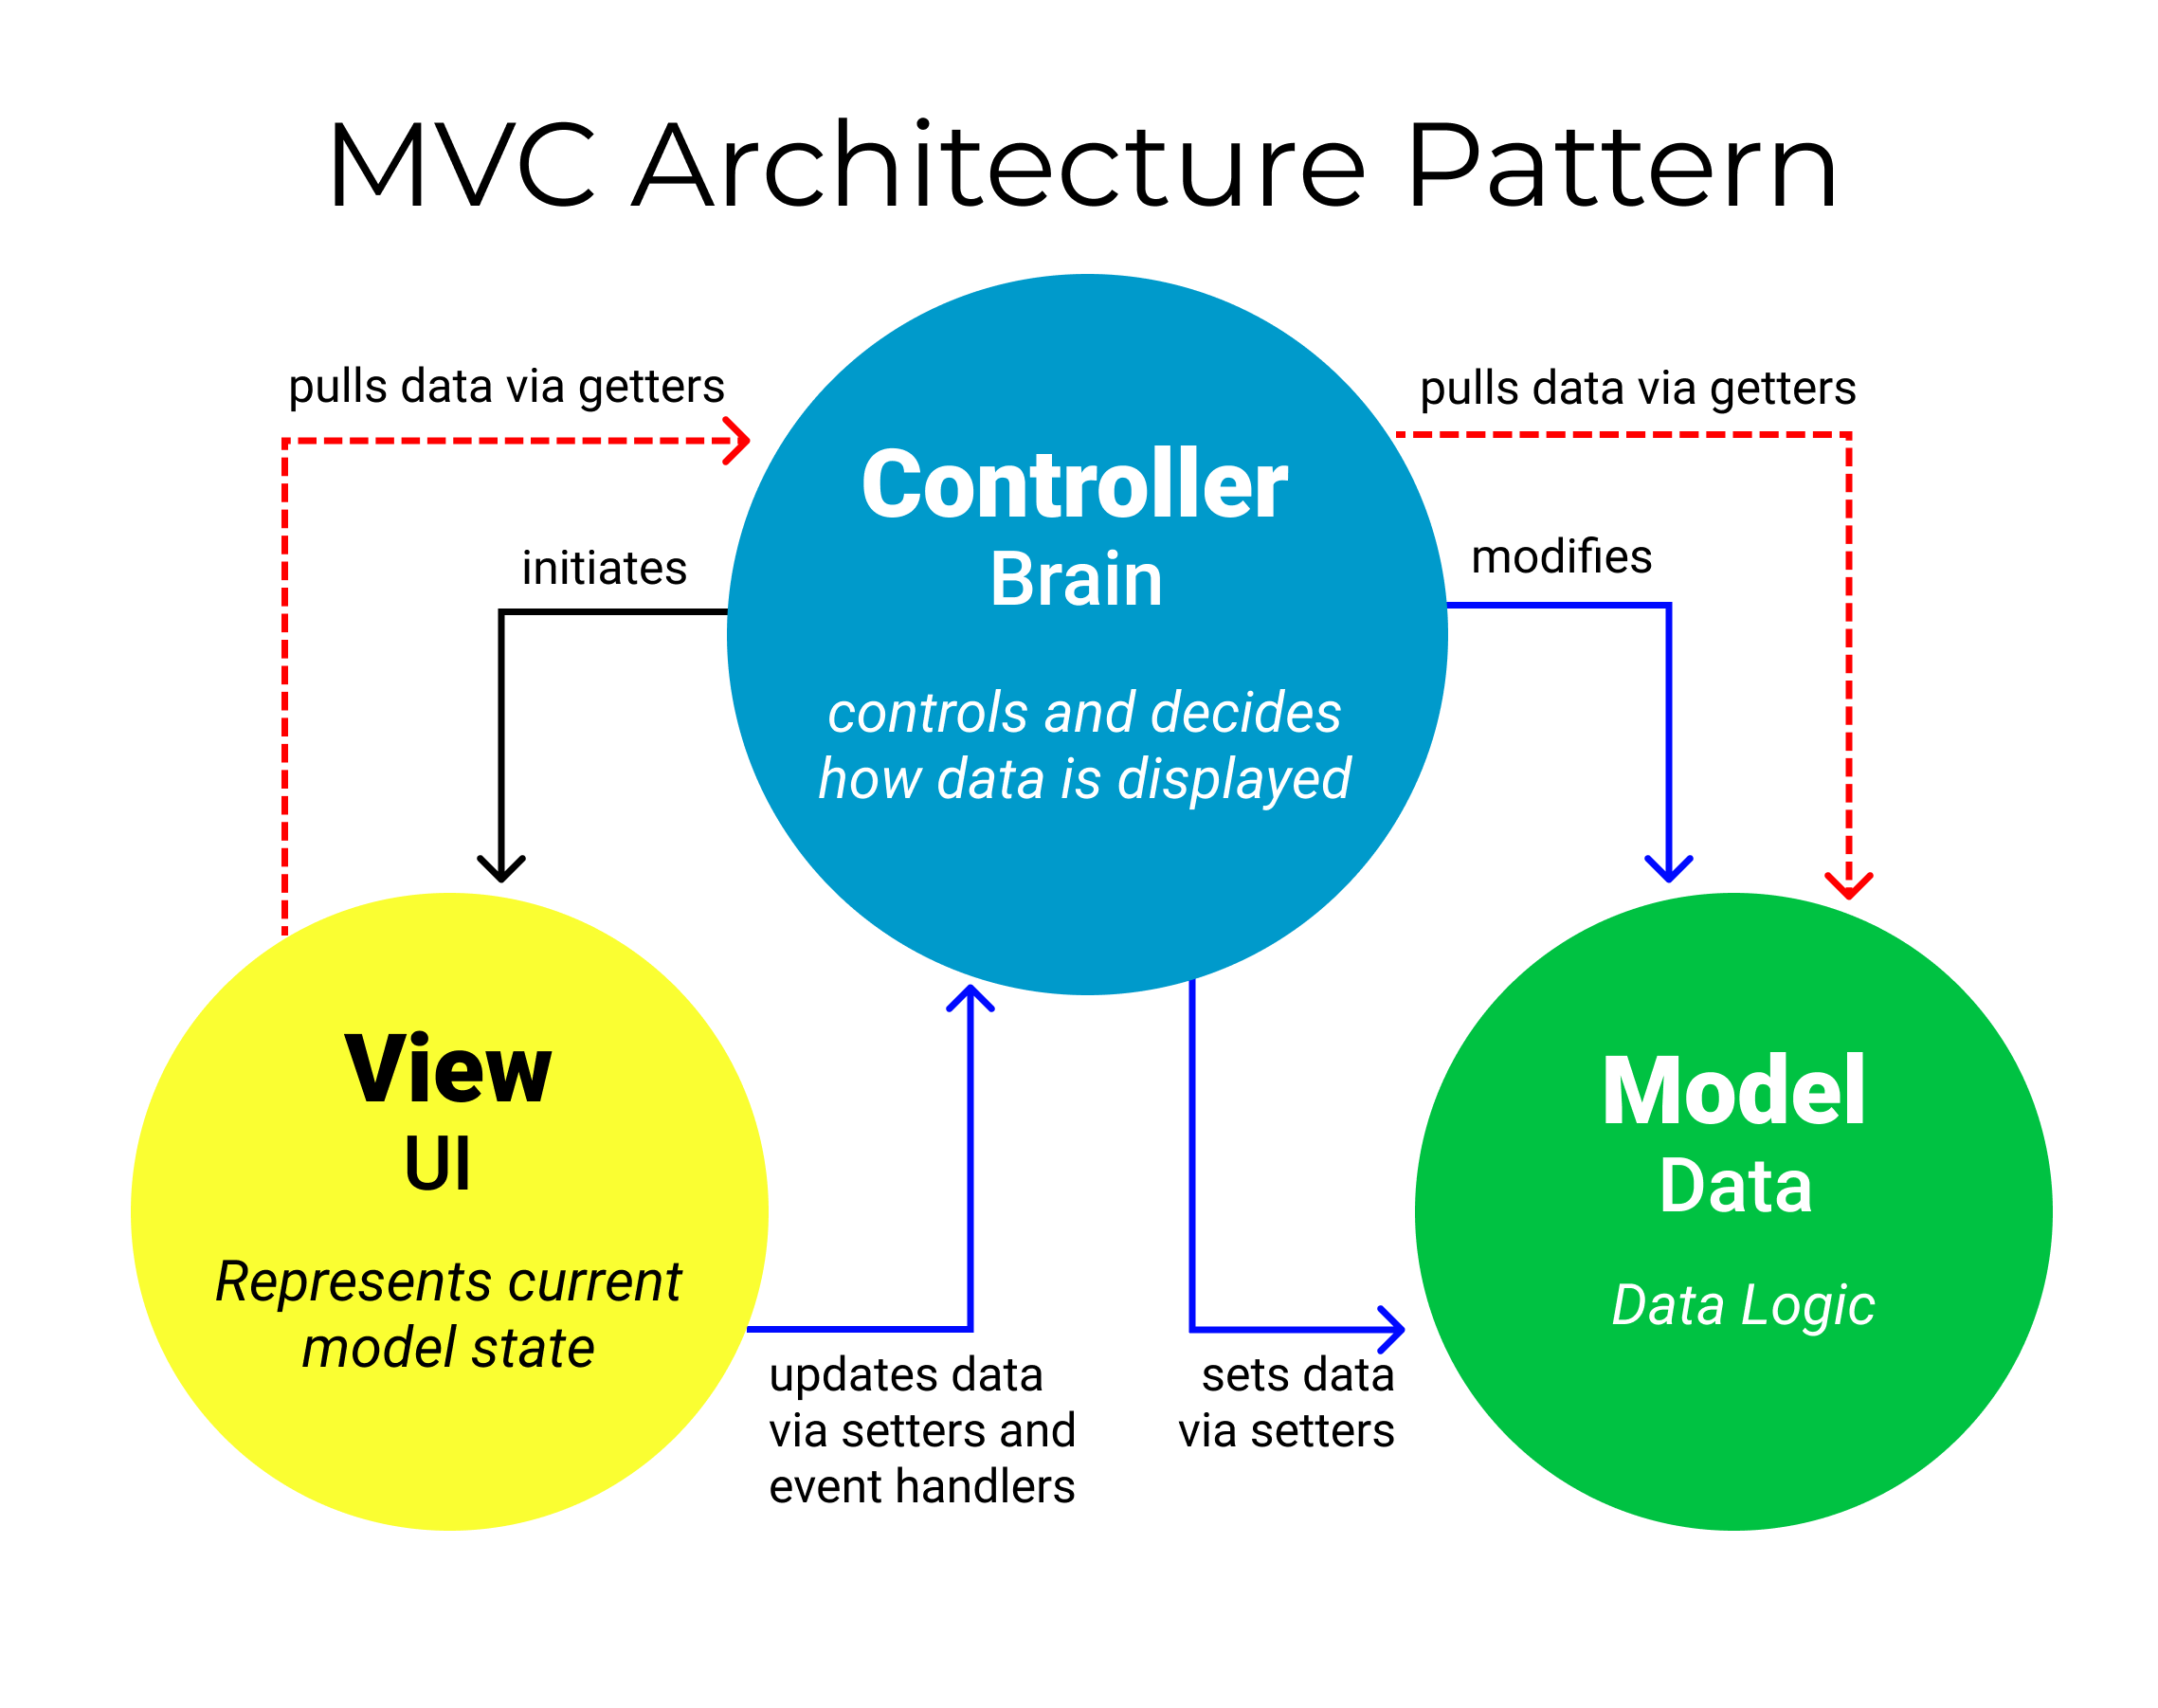
\includegraphics[width=.5\textwidth]{Graphics/MVC3.png}
\end{figure}

Som en tilføjelse, der ikke vil indgå i den endelige aflevering, og som ikke indgår i eksekveringen af de tre klasser for oven, laver vi også en board-driver klasse, der vil være i stand til at kunne teste "board" klassens funktionsdygtighed. Dette gør vi, eftersom der ikke vil være mulighed for at teste logikken rent visuelt, før controller/scene-builder delen er færdig. Dette skyldes, at controller-klassen modtager og arbejder med data fra board, og hvis controllerklassen så ikke er færdig, er den ikke i stand til at gøre dette på en ordentlig måde. 

\subsection{Board Design}

% !TeX root = ..\G16.tex
\section{Implementering}

\subsection{Board}\label{sec:boardImplement}
Modellen for brættet implementeres i \mintinline{java}|Board.java| klassen. \cref{tbl:boardfields} indeholder klassens felter.
\begin{table}[H]
    \centering
    \caption{Felter i \mintinline{java}|Board.java|}\label{tbl:boardfields}
    \begin{tabular}{ll}
        \toprule
        Felt                                                              & Formål                                           \\
        \midrule
        \mintinline{java}|int[][]board|                                   & Datastruktur der repræsenterer brættet.          \\
        \mintinline{java}|int turnCount|                                  & Turnummeret i spillet                            \\
        \mintinline{java}|int boardsize|                                  & Størrelsen \(n\) for et \(n\times n\) bræt.      \\
        \mintinline{java}|int forfeitCounter|                             & Antal gange en spillerne har meldt pas           \\
        \mintinline{java}|ArrayList<int[]> flipped|                       & Log over de sidste vendte brikker                \\
        \mintinline{java}|HashMap<Integer, String> players|               & Spillernes interne ID og navne                   \\
        \mintinline{java}|HashMap<String, HashMap<Integer,|               & Datastruktur for mulige træk for en given farve, \\
        \quad \mintinline{java}|HashMap<Integer, Integer[]>>> validMoves| & en given tur.                                    \\
        \bottomrule
    \end{tabular}
\end{table}
Brættet repræsenteres af en heltalsmatrix med værdierne \(0\) for tomt felt, \(1\) for hvid placering og \(2\) for sort placering. Ved at gemme turnumre og antal gange spillere har meldt pas kan board klassen afgøre hvis tur det er og om spillet er slut.
Loggen over vendte brikker endte med ikke at blive brugt, men formålet var at kontrollerklassen skulle vise hints om hvilke brikker der ville blive vendt ved et givent træk. Det blev stemt ned da det gør spillet for nemt.\newline
\cref{tbl:boardmethods} indeholder klassens metoder.
\begin{table}[H]
    \centering
    \caption{Metoder i \mintinline{java}|Board.java|}\label{tbl:boardmethods}
    \begin{tabular}{ll}
        \toprule
        Metode                                                        & Formål                                                                               \\
        \midrule
        \mintinline{java}|Board()|                                    & Konstruktør for brættet. Kalder \mintinline{java}|setPlayers()|.                     \\
        \mintinline{java}|getBoard()|                                 & Getter for board feltet.                                                             \\
        \mintinline{java}|setPiece(int row, int column, int colour)|  & Sætter manuelt brik, uanset lovlighed.                                               \\
                                                                      & Bruges til unit tests.                                                               \\
        \mintinline{java}|getTurn()|                                  & Getter for turnCount.                                                                \\
        \mintinline{java}|turnClock()|                                & Inrementere turnCount.                                                               \\
        \mintinline{java}|getPlayers()|                               & Getter for spiller hashmap.                                                          \\
        \mintinline{java}|getValidMoves()|                            & Getter for validMoves hashmap.                                                       \\
        \mintinline{java}|setPlayers()|                               & Tildeler tilfældigt spillere en farve.                                               \\
        \mintinline{java}|setPlayers(int id1, String player1,|        & Tildeler spillere specifikke farver.                                                 \\
        \quad \mintinline{java}|int id2, String player2)|             &                                                                                      \\
        \mintinline{java}|setPlayerName()|                            & Setter for specifikt spillernavn.                                                    \\
        \mintinline{java}|resetBoard()|                               & Nulstiller brættet, turnummer og pastæller.                                          \\
        \mintinline{java}|turnState(int colour)|                      & Kalder \mintinline{java}|moveAnalyser(colour)|,                                      \\
                                                                      & og udregner om der er ledige træk.                                                   \\
        \mintinline{java}|gameOver()|                                 & Afgør om spillet er slut hvis brættet er fyldt,                                      \\
                                                                      & eller der er meldt pas to gange i træk.                                              \\
        \mintinline{java}|initPlace(int row, int column, int colour)| & Indeholder logik for at udfylde startfelterne (midterste firkant).                   \\
        \mintinline{java}|place(int row, int column, int colour)|     & Placere en brik hvis placeringen er tom og indeholdt i validMoves.                   \\
                                                                      & Kalder \mintinline{java}|flip(move, colour)|.                                        \\
        \mintinline{java}|flip(String move, int colour)|              & Vender brikker ved et lovligt træk.                                                  \\
        \mintinline{java}|filled()|                                   & Afgører om brættet er fyldt.                                                         \\
        \mintinline{java}|checkWinner()|                              & Tæller brikker og afgører vinderen.                                                  \\
        \mintinline{java}|moveAnalyser(int colour)|                   & Gennemgår ledige felter og afgør og de er lovlige træk (se \cref{sec:moveAnalyser}). \\
        \mintinline{java}|findOwn(int[][] checkboard, int i,|         & Afgører om et træk resulterer i indkapsling af modstanderen.                         \\
        \quad \mintinline{java}|int j, int direction, int colour)|    &                                                                                      \\
        \mintinline{java}|saveFlips(int[] ownPiece, int i,|           & Gemmer indkapslede brikker.                                                          \\
        \quad \mintinline{java}|int j, int direction)|                &                                                                                      \\
        \bottomrule
    \end{tabular}
\end{table}

\subsection{Main}

\subsubsection{Basic}

\subsubsection{Avanceret}

\subsubsection{FXML}\label{BD}
Brættet er lavet af en 8x8 gridpane med en pane i hver celle. Hver pane indeholdt i gridpanes cellen er tildelt et unikt id. For eksempel er 05 et unikt id tildelt til en pane, hvor 0 repræsenterer rækkeindekset, og 5 repræsenterer kolonneindekset for panes placering i gridpane. Hver pane er tildelt et id for at gøre det nemmere at placere/tegne eller slette en brik fra brættet.


\subsection{Controller}

\subsubsection{Basic}



\subsubsection{Avanceret}
I den avancerede controller klasse er der rykket om på rækkefølgen, hvori metoderne kaldes.
\begin{table}[H]
\centering
\caption{}\label{tbl:}
\begin{tabular}{lllll}
\toprule
Metode & Kalder metoderne: & Beskrivelse & Input & Output \\
\midrule
beginGame() & setName() & Sætter hele spillet i gang & ActionEvent event & Ting 4 \\
&& og loader spillebrættet \\
& \\

setName() & setNameBtn() & Beder spillerne om \\ 
& checkScore() & at indtaste deres navne \\
&& i tekstfelterne og \\
&& sætter deres score lig 0\\
& \\

setNameBtn() & in() & fastlåser spillernes navne \\
&& og sætter spillet i gang\\
& \\

in() & drawCircle() & tildeler spillerne deres \\
&& farver og viser de fire \\
&& første mulige træk \\
& \\

firstFour() & update() & Får spiller til at sætte \\
& checkscore() & de fire første brikker\\
& \\

onPaneClicked() & getRowIndex() & Styrer hvad der sker, når \\ 
& getColumnIndex() & der bliver klikket på et felt\\
&  firstFour() & Giver spillerne besked, om \\
& hideLegalMoves() &hvorvidt deres træk er lovlige\\
& update() & Melder pas, når der \\ 
& checkScore() & ikke er noget lovligt træk\\
& showLegalMoves() & Annoncerer spillets slutning,\\ 
&& når der ikke er \\
&& nogen lovlige træk tilbage\\
& \\

gameOver() & loadHighScore() & Erklærer vinderen\\
& checkHighScore() & og opdaterer high-score'n\\
&& (hvis den er blevet slået) \\


\bottomrule
\end{tabular}
\end{table}

\begin{table}[H]
\centering
\caption{}\label{tbl:2}
\begin{tabular}{lll}
\toprule
Metode & Kaldte metoder & Beskrivelse  \\
\midrule
restart() & reset() & Genstarter spillet og beder spillerene om   \\
& setName() & at indsatte deres navne  i tekstfelte igen.  \\
& & Spiller der lavet første træk i  \\
& & sidste runde, begynder anden \\
\\
reset() & & Iterer gennem brættet og rydder det \\
\\
update() & drawCircle() & Opdatere brættet og tegner circkler(brikker)  \\
& & på brættet ifølge Board objektet \\
\\
exitGame() \\
\\
checkScore()& & Opdaterer scoren for begge spillere\\
\\

saveHighScore() & & Gemmer vinderens score og navnet adskilt af \\
& &  komma inde i "Highscore.txt" file, hvis vinderens  \\
& & score er højre end nuværende highscore\\
\\
loadHighScore() & & Læser highscore og spillersnavne fra \\
& & "Highscore.txt" filen og retunere de som arrayet.\\
\\
showHighScore() & loadHighScore() & Når man trykker på highscore-knappen, \\
& & vises en advarselsboks/-prompt, der viser highscore  \\
& & og spillerens navn, hvis highscore er indstillet. \\
\\

surrender() & & Annoncere overgivelsen af den spiller\\
& & der trykkede på knappen,\\
 & & og den anden spillers sejr\\
\\
getRowIndex()& & Returnerer rækkeindekset for pane, der er klikket på\\
\\
getColumnIndex()& & Returnerer søjleindekset for pane, der er klikket på\\
\\
showLegalMoves() & drawCircle() & Tegner en cirkel hvor spiller kan \\
hideLegalMoves()\\
mainMenu()\\

\bottomrule
\end{tabular}
\end{table}

% !TeX root = ..\G16.tex
\section{Test}
Når vi skulle teste programmet, havde vi forskellige tilgange til det, alt efter hvad vi arbejdede med. Os, der arbejdede med det visuelle, skulle bare åbne programmet og se, om vi var tilfredse med overfladen, og om de diverse knapper gjorde som de skulle, når vi klikkede på dem. Vi skulle ikke arbejde med nogen kompliceret logik. 
\subsection{Board-driver klassen}
Board-driver klasse, der vil være i stand til at kunne teste "board" klassens funktionsdygtighed. Dette gør vi, eftersom der ikke vil være mulighed for at teste logikken rent visuelt, før controller/scene-builder delen er færdig. Dette skyldes, at controller-klassen modtager og arbejder med data fra board, og hvis controllerklassen så ikke er færdig, er den ikke i stand til at gøre dette på en ordentlig måde.
\subsection{Unit tests}\label{sec:unitTests}
For at tilgodese at Board klassens logik virker efter ændringer blev en testklasse, \mintinline{java}|BoardTest.java| skrevet som kører hver gang et jar-arkiv kompileres eller klassen køres. Testen tester setter og getter metoder for player hashmappet, moveAnalyser og turnState metoderne.
% !TeX root = ..\G16.tex
\section{Project Management}\label{sec:pm}
I følgende afsnit vil der blive diskuteret de valgte løsninger til at organisere projektet og løse opgaven.
\subsection{Tidsplan og tidsstyring}
Indledningsvist blev gruppen enige om en række principper og en tidsplan for at optimere udviklingsplanen. Principperne lyder:
\begin{enumerate}
    \item Nær-daglig status på underopgaver.
    \item Alle planer er tentative.
    \item Fælles udvikling af logik og algoritmer i vigtige metoder.
\end{enumerate}
Den oprindelige tidsplan kan ses i \cref{fig:gantt}.
\begin{figure}[H]
    \centering
    \caption{Første tidsplan (fra Projektplanen)}\label{fig:gantt}
    \begin{ganttchart}[
            % expand chart = \textwidth,
            hgrid,
            vgrid,
            time slot format = isodate,
            % inline,
            % milestone inline label node/.append style={left=5mm},
            % milestone/.append style={xscale=.5},
        ]{2023-01-04}{2023-01-20}
        \gantttitlecalendar{month=shortname, day} \\
        \ganttgroup{BasicReversi}{2023-01-04}{2023-01-11} \\
        \ganttbar{Logisk model}{2023-01-04}{2023-01-06} \\
        \ganttbar{GUI implementering}{2023-01-04}{2023-01-10} \\
        \ganttbar{Test af BasicReversi}{2023-01-11}{2023-01-11} \\
        \ganttmilestone{BasicReversi færdig}{2023-01-11} \\
        \ganttgroup{AdvancedReversi}{2023-01-11}{2023-01-16} \\
        \ganttbar{Test af AdvancedReversi}{2023-01-17}{2023-01-18} \\
        \ganttmilestone{AdvancedReversi færdig}{2023-01-18} \\
        \ganttgroup{Rapportskrivning}{2023-01-04}{2023-01-20} \\
        \ganttbar{Rapportafslutning}{2023-01-19}{2023-01-20} \\
        \ganttmilestone{Aflevering}{2023-01-20}
    \end{ganttchart}
\end{figure}
Under projektet overholdte vi ovennævnte principper, men tidsplanen ændredes markant. BasicReversi var færdig to dage over tid og rapportskrivningen blev lempeligt udskudt til den sidste uge.
\subsection{Arbejdsfordeling}
I forhold til arbejdsfordelingen er projektet opdelt i tre faser:
\begin{enumerate}
    \item Logik \& Brugerflade
    \item Controller klassen
    \item AdvancedReversi funktionaliteter
\end{enumerate}
I første fase arbejder gruppen i makkerpar. To personer nærstudere JavaFX og prøver at implementere den ønskede brugerflade og giver deres \emph{concerns} til det andet makkerpar. Det andet makkerpar arbejder på at implementere logikken bag brættet og brikkerne i en model klasse.\newline
I anden fase arbejder gruppen sammen på at løse forskellige problemstillinger. En kunne f.eks. arbejde på den overordnede struktur af metodekald i et spil Reversi, en anden arbejder på at oversætte museklik til koordinater, en tredje arbejder på reaktioner fra knapper, og en sidste på opdatering af det grafiske bræt ud fra den interne tilstand af bræt objektet. Til sidst en større sammenfletning som leder til en controller klasse, og efter test af spillet, et færdigt produkt.
I tredje fase bliver det oprindelige spil forgrenet via Git og hvert gruppemedlem implementerer et af gruppens tilføjelser af gangen. Når en implementation er færdig flettes denne med hovedgrenen. Her er der valgt en person som mestendels arbejder med at flette de forskellige grene sammen.
\subsubsection {Basic}\label{PBS}
Måden vi valgte at arbejde på i den Basic-Reversi havde både fordele og  ulemper. \newline
Fordele: 
\begin{itemize}
\item At fokuserer på de tildelte metoder så man kan går helt i dybden med disse fejl man møder under processen, samtidig med at forberede sig til en forklaring på det til de andre gruppemedlemmer, så alle er med på opdateringer i forbindelse med metoden og de løsninger man bringer med hvis man oplever nogle fejl,hvilket også føret til at styrke sammenarbejde og kommunikation i gruppen.
\end{itemize} 
 Ulemper:
\begin{itemize}
\item Hvert medlem har sat mere fokus på de tildelt/valgte metoder som man have ansvar for, hvilket gør at man ikke sætter ligevægt på alle processorerne i projektet. Vi talte bestemt med hinanden om alle faser og gav tilstrækkelige forklaringer på de ideer og koder, der blev brugt, samt løsninger, hvis der var fejl, men det opnåede læring vil ikke være på samme niveau, som hvis vi havde arbejdet sammen på alle faser med samme effektivitet. 
\end{itemize}
\subsubsection {Advanced}\label{PAC}
Avanceret del bajet på at udvikle noget vi allerede har, eller tilføj nye funktioner hvor man synes at det kunne være interessant for spiller, og som gør spillet mere effektiv.
Måden vi har arbejdet på i den avanceret del, var lidt mere individuelt end Basis. 
Vi begyndte at tale om de forskellige idéer vi havde. Derefter gik vi i gang med de udvalgte idéer, da alle har en idé eller to at arbejde videre med.
Der har været lidt mere plads til at arbejde med de faser som man ikke havde i Basis del, fx Yahya og Rasmus havde hoved ansvar for logikken (Board class) i den Basis version, hvor imod den avanceret, valgte Yahya at arbejde mere med Design ” main.FXML”, hvor han tog en del af Design Udviklingen, hermed (farver, knapper, størrelser, tekster), for at komme ind på detaljer og lærer SceneBuilder bedre at kende.







\subsection{Git, Github og Gradle}\label{sec:GGG}
Som projektstyringsværktøjer er der valgt følgende løsninger:
\begin{itemize}
    \item \faGit \ \href{https://git-scm.com/}{Git}: Til at kommunikere mellem lokale maskiner og \href{https://www.overleaf.com/}{Overleaf}, hvor rapporten kan skrives i fællesskab.
    \item \faGithub \ \href{https://github.com/}{Github}: Til at håndtere versionskontrol mellem medlemmer i gruppen.
    \item \href{https://gradle.org/}{Gradle}: Projektstyringsværktøj til at automatisere \emph{dependencies} (JavaFX), mappestrukturer og pakning af jar-filer.
\end{itemize}
\subsubsection{Git og Github}
Som nævnt i \cref{sec:introtilg} er projektet på Github \href{https://github.com/rwiuff/Reversi}{https://github.com/rwiuff/Reversi} \github{https://github.com/rwiuff/Reversi}. Dette \emph{repository} (repo) er udgangspunkt for versionskontrol i projektet. Desuden bruges Overleafs Git integration til at synkronisere projektet med lokale maskiner. Git som versionstyringsprogram har været essentielt under projektet. Der har været meget læring i at bruge \emph{branch} og \emph{merge} funktionerne til at kunne arbejde på forskelige aspekter af kode i de samme klasser på samme tid. Det har mestendels været uden de største problemer, men der er til stadighed meget mere at lære om samarbejde med VCS.
\subsubsection{Gradle}
Via Gradle kan mappestrukturen i \cref{fig:tree} genereres. Mappestrukturen indeholder desuden også bin og build mapper som bruges under kompilering og pakning af jar-arkiver, men disse er kun midlertidige instanser af det program man kører.
\begin{figure}[H]
    \caption{Mappestrukturen i JavaFX projekterne BasicReversi og AdvancedReversi}\label{fig:tree}
    \dirtree{%
        .1 BasicReversi / AdvancedReversi \ldots{} \begin{minipage}[t]{6cm} Rodmappen indeholder \emph{gradlewrapper} og \emph{settings.gradle} \end{minipage}.
        .2 app \ldots{} \begin{minipage}[t]{5cm} \emph{build.gradle} \end{minipage}.
        .3 src.
        .4 main.
        .5 java.
        .6 basicreversi / advancedreversi \ldots{} \begin{minipage}[t]{5cm} \mintinline{java}|.java| klasser \end{minipage}.
        .5 resources.
        .6 basicreversi / advancedreversi \ldots{} \begin{minipage}[t]{5cm} Billedfiler og \mintinline{java}|.fxml| filer \end{minipage}.
        .4 test.
        .5 java.
        .6 basicreversi / advancedreversi \ldots{} \begin{minipage}[t]{5cm} Testklasser \end{minipage}.
        .2 gradle.
        .3 wrapper \ldots{} \begin{minipage}[t]{5cm} Indeholder wrapper filer \end{minipage}.
        .2 releases \ldots{} \begin{minipage}[t]{10cm} Indeholde de færdige jar-arkiver \end{minipage}.
        }
\end{figure}

Gradle tilgodeser automatisk udførsel af skrevne tests, håndtering af kompilerede .class filer og pakning af jar arkiver. Desuden tilgodeser Gradle at dependencies er tilgængelige for miljøet der åbner projektet, uden at man skal importere JavaFX moduler manuelt. Er der en fejl i den version af JavaFX der bruges, kan man blot opdatere versionsnummeret i \emph{build.gradle} og herefter opdateres JavaFX.


% !TeX root = ..\G16.tex
\section{Konklusion}

\subsection{Vores mål}\label{VM}
Vi satte os til mål at skulle skrive programmet Reversi i sin mest basale form. Dette opnåede vi, og dermed opfyldte vi vores minimums-krav. Dernæst satte vi for os selv, at vi ville lave så mange avancerede tilføjelser til programmet som muligt. Vi nåede at tilføje flere udvidelser, som forbedrede spillerens brugeroplevelse, hvilket var en sejr, men der var også forsøg på udvidelser, hvor vi måtte se os slået. Se næste {vores mangler} for yderligere info. 
Vores kode endte med at være let overskueligt og struktureret. Vi var i stand til at implementere flere udvidelser, enten via. genbrug af kode fra den basale kildekode, eller ved indsættelse af ny kode enkelte steder, uden at forpurre systemet. Ofte kunne vi ganske enkelt oprette en metode, og så kalde den de steder, hvor det var relevant. 
Vi lærte også at arbejde som en gruppe inden for software/programmerings-feltet. De fleste af os var nye til brugen af "Git-Hub", men takket være Rasmus' erfaring og kyndighed med programmet, lærte vi hurtigt hvordan vi kunne arbejde sammen, dele kode, push'e, pull'e, og skabe nye grene, hvorpå vi kunne arbejde på vores udvidelser i fred, uden nogen uventede ændringer i koden. 


\subsection{Vores mangler}
\subsubsection{SpeedReversi}\label{SR}
En pointe fremhævet i den avancerede del af Yahya, er, at give spillere mulighed for at spille med en timer.
\begin{itemize}
\item Timeren er en vigtig del af de fleste strategispil (spil, der kræver en vis forhånds- planlægning til næste træk), fordi timeren øver spillernes tænkehastighed og tvinger dem til at tænke hurtigere og træffe beslutninger for næste træk under pres, hvilket kan føre til at man træffer en forkert beslutning, eller at man løber tør for tid. Denne tilføjelse til denne type spil gør spillet sjovere for nogle. 
\end{itemize}

I gruppen aftalte vi at Yahya starter med at implementere timer-metoden ind i vores standard logik og får den til at køre direkte, når spillet starter. Derefter vil vi så tilføje en Bottom til ”menu.fxml” kaldet: ” Speed-Reversi ”, der finder plads under ”BeginGame” (normal game).
På den måde adskiller vi ”SpeedMode”, så det bliver et ekstra valg hvis man ønsker det. 
Timer-Metoden tog ca. 2 dage at implementere, for der har været nogle udfordringer undervejs så som: 
\begin{itemize}

\item Der blev brugt "Thread" til at manipulere timeren med spillet, men fejlen var at ved brug af "Thread.sleep" vil det tage programmet et sekund at kører metoden igennem. Det har vi oplevet, da vi har prøvet at spille hurtigt; så vil timeren ikke begynde på at tælle ned, for den har brug for et sekund til at tænke. 
\item Som et forsøg på at løse fejlen, har vi prøvet at forkorte rundturstiden for "Thread.sleep" ved at bruge "System.nanoTime" hvor man kan regne tiden, som metoden bruger i nanoTime, og trække det fra. Det hjalp ikke; fejlen var det samme. 
\item Et andet forsøg, var ved at prøve "Animationtimer" men vi kunne ikke få metoden til at ændre timeren fra spiller 1 til spiller 2. 
 i 
\item Løsning: 
Der blev brugt "TimeLine" hvor den virkede fint med både "turnsskift"-hastighed mellem spillerne og reagerer med "getturn()". 
\end{itemize}
\subsubsection{Flette Reversi-Timer}\label{FRT}
Nogle af de største udfordringer vi har haft med SpeedMode er, at kombinere metoden ind og få den til at køre adskilt, dvs. kun når man vælger at spille med SpeedMode, som vi har lavet en knap til i "Menu.FXML" og en "BorderPane" i "Main.FXML".
\subsubsection{Metodeimplementering}\label{MI}
\begin{itemize}
\item Efter oprettelsen af "ReversiTimer"-klassen, som indholder Timer-metoden, har Yahya tænkt sig at oprette en anden Controller-klasse for ReversiTimeren, således at man kan kaldee den nye "controller1" når man trykker på knappen " SpeedReversi" ellers kaldes den nuværende "Controller".
På den måde vil vi nemt kunne flette Timer-logikken ind med standard logik uden væsentlige ændringer i koden, men der har været uenighed om det, for det kunne være et problem, hvis vi senere opdager nogle fejl eller hvis vi skal ændre på noget i hoved-Controller-klassen, for så bliver vi nødt til også at ændre det i Controller2-klassen. 
\item Derfor havde vi tænkt os at få Timeren ind ved at tilføje en "boolean" som sætter "SpeedMode=false;" og så begyndte vi at tilføje 
" if (speedMode == true) \{ " "else" til metoderne ( in(),restart(),onPaneClicked(),beginGame) og så satte vi 
"speedReversi(ActionEvent event) \{	
		speedMode = true; "
\item Vi var meget tætte på at få det hele til at køre, men udfordringer var stadig til stede. Vi mødte en fejl, der gør at enten kan timeren ses på begge "modes", ellers forsvinder den i begge Mode også, dvs. at der har været en sammenhæng mellem den normal logik og den ny med Timeren.
Efter en lang analyse af "if" og "else" sætninger fandt vi fejlen, som var bag 'Controller', da vi loadede "main.fxml" med standard Controller'en hver gang, derfor vil 'Value' af SpeedMode altid være "True". 

\item Løsning: 
implementere følgende i "speedReversi(ActionEvent event)":
\item kald metoderne fra "begingame()" med følgende tilføjelser 
" controller.setSpeedMode(true);
            controller.getReversiTimerpane().setVisible(true); " 

   sæt følgende metoder ind i "begingame"
   " controller.setSpeedMode(false);
        controller.getReversiTimerpane().setVisible(false); "

\item Dette opnåede rettelser var desværre forsent til at kunne flette ind i hoved projekt, som vi fik at vide at sene ændringer kan kost dyrt. Derfor valgt vi at leverer den bedste version vi kunne nå til den tid vi har. 
\end{itemize}








\subsubsection{Antal Mulige vendinger}\label{AMV}
Aslan forsøgte sig med en udvidelse til udvidelsen, der gjorde spillerne i stand til at se deres mulige træk. Idéen med udvidelsen var den, at man kunne ved at trykke på en knap, kunne se på de mulige træk, hvor mange brikker der vil blive vendt. Altså hvis man ved at sætte en brik på en mulig placering, vil vende 3 brikker, vil der stå tallet 3 i midten af den mulige placering. Problemet ved implementeringen opstod, da programmet skulle se fremad, fremfor bagud. Strategien var, at skabe en integer i board-klassen, kaldet "tilesFlipped". Hver gang metoden 'flip()' blev kaldt, skulle denne integer sættes lig 0, og jeg satte den til at inkrementere hver gang en brik blev vendt, således at man altid vil få det eksakte tal vendte brikker. Dernæst modificerede jeg 'showLegalMoves' til at vise 'tilesFlipped' i midten af cirklerne. Problemet var følgende: For det første, viste alle cirkler det samme tal. Derudover viste cirklerne altid hvor mange brikker der blev vendt SIDSTE runde. Målet var, at de skulle vise tallene en runde FREMAD. Forsøgene nåede deres ende, ikke på grund af fejl og exceptions, men ganske enkelt grundet en blokade. Jeg havde ingen anelse om, hvor jeg skulle implementere hvad. Nøglen lå i board-klassens 'validMoves', men grundet min manglende erfaring med hashmaps, som board-klassen i høj grad består af, så jeg mig nødsaget til at give op. 

\subsubsection{Lyd}\label{lyd}
Lyd er en af de andre avancerede funktioner, som Abinav forsøgte at implementere. Lyd ville forbedre brugeroplevelsen og hjælpe spillere med at fordybe sig i spillet, hvilket gør det til en fremragende funktion at inkludere. Efter hvert træk ville funktionen have ladet deltagerne vide, hvordan spillet forløb. Derudover ville det have givet spillerne feedback om, hvorvidt de havde placeret brikken korrekt på brættet. At inkludere lyd i spillet ville have mindsket behovet for, at spillere skulle læse teksten efter hvert træk, eller mens de placerede brik på brættet.
Musikfilerne blev importeret ved hjælp af Java FX-værktøjer som mediaPlayer og media. Fejl som fil kan ikke findes, og fil kan ikke indlæses, blev stødt på under adgang til mediefiler. Try-catch-sætninger blev brugt til at rette op på disse problemer. Hver lyd- eller mediefil havde en separat metode, der indeholdt funktionerne mediaPlayer.play(), mediaPlayer.stop() og mediaPlayer.stop(). De nævnte teknikker gjorde det muligt at afspille, pause og stoppe musikken. Det vigtigste problem, der opstod under integration af lydkomponenten, var, at musikfilerne af og til, når programmet kørte, ville blive korrupte. Musikfilerne fungerede korrekt, når de blev afspillet ved hjælp af VCL eller groove-musik på computeren. Det var umuligt at afgøre, hvad der fik musikfilerne til at blive korrupte, da programmet kørte. Et andet problem, der udviklede sig, var lydens manglende evne til altid at spille som reaktion på brugerens aktivitet. Der var adskillige forsøg på at rette denne fejl, herunder at kontrollere, om handlingshændelsens kode kaldte den relevante lydfil, men ingen af dem lykkedes. Til sidst blev det besluttet ikke at tilføje funktionen lyd til Reversi, da de fejl, der blev opstået ved at tilføje funktionen, ikke var i stand til at rette og krævede et højt kendskab til java fx mediaplayer og medieklasse.


\subsection{Hvad har vi lært}
\subsubsection{Aslan}\label{HHVLA}
Dette projekt har bidraget meget til mit billede af, hvordan det er at arbejde inden for software/programmeringsfeltet. Jeg var i begyndelsen meget usikker på, hvordan man skulle arbejde som gruppe på ét projekt, da vi tidligere afleveringsopgaver ganske enkelt har delt de fire forskellige opgaver op imellem os. Jeg fandt dog hurtigt ud af, at systemet er det samme, og dog ikke. Man uddelegerer opgaver, men sparer også meget med hinanden, og kigger på tingene sammen. Man arbejder på at forbedre hinandens arbejde, så man i fællesskab kan komme frem til det bedst-mulige produkt. Derudover har dette forløb også bare været en god mulighed for at udvikle mine programmerings- og problemløsningskompetencer. Det har været fedt at kunne stå over for et problem, og have muligheden for at teste forskellige løsninger af døgnet rundt, frem for at skulle bekymre sig om andre fag. Jeg håber på flere forløb som dette i fremtiden, hvor vi alle er mere erfarne og kompetente programmører.  
\subsubsection{Yahya}
\subsubsection{Rasmus}

\subsubsection{Abinav}\label{AA}


%Bibliography herunder:
%\newpage

%\bibliographystyle{unsrtnat}
%\bibliography{Bibliography}

\newpage
\listoflistings
\addcontentsline{toc}{section}{Listings}
\newpage
\listoffigures
%\newpage
%\renewcommand{\listtablename}{Liste over huskeord}
\listoftables
\newpage

% Appendicer herunder:

% !TEX root = G16.tex
\appendix
\appendixpage
\addappheadtotoc
\section{Afsnitsforfattere}\label{sec:arbejde}
\cref{tbl:arbejde} viser en oversigt over hvilke gruppemedlemmer der har skrevet hvilke afsnit i rapporten.
\begin{table}[H]
    \centering
    \caption{Forfatterskab i rapporten}\label{tbl:arbejde}
    \begin{tabular}{p{.48\textwidth}p{.48\textwidth}}
        \toprule
        Navn            & Afsnit                                \\
        \midrule
        Abinav Aleti    &                                       \\
        \midrule
        Yahya Alwan     &                                       \\
        \midrule
        Aslan Behbahani & \cref{MS,OP,TTO,MVC}                  \\
        \midrule
        Rasmus Wiuff    & \cref{sec:introtilg,sec:speci,sec:pm} \\
        \bottomrule
    \end{tabular}
\end{table}

\end{document}
